\chapter{Background}

%\textit{Note: Describe each proven technology / concept shortly that is important to understand your thesis. Point out why it is interesting for your thesis. Make sure to incorporate references to important literature here.}

The psychological process of finding reasons behind a behaviour happens naturally and often unawarely. In the early attempts of studying attribution, Heider \cite{Heider1958} even considers people naive psychologists, who try to make sense of the causes and effects of various happenings. Therefore, this chapter dives deeper into the research surrounding attribution, as it is the base motivation for this thesis. We will start with the basics, covered in \textit{\nameref{PsychologicalBackground}}, and conclude with more specific insights on the intersection between attribution and software engineering in \textit{\nameref{DisAttSE}}. 


\section{Psychological Background} \label{PsychologicalBackground}

\textit{Attribution} is not only the first word in the title of this thesis; it also constitutes the core subject under study. As human beings, we are forming attributions everytime we ask "why" and try to find an answer that argues the cause of an event. The theory that is concerned with studying attributions is known as \textit{Attribution theory} and can be best described through the following definition: 

\begin{quote}
“Attribution theory deals with how the social perceiver uses information to arrive at causal explanations for events. It examines what information is gathered and how it is combined to form a causal judgment”. \cite{Fiske1991}
\end{quote}

There are various streams of research that have emerged, but we want to focus on one of the most substantial works in attribution theory, Heider's \textit{The psychology of interpersonal relations}, which considers the cause of a behaviour to be either internal (e.g., a disposition or a characteristic of a person) or external (e.g. an environmental factor). These are often referred to also as dispositional and situational attribution. 

One of the major areas of interest in the attribution literature concerns the cognitive processes that lead from observation of behaviour to dispositional attribution \cite{Trope1989}. Trope even constructed a two-stage attribution model. This model fundamentally indicates that dispositional attribution is positively related to the identification of the corresponding behaviour and negatively related to the identification of the corresponding situational inducements \cite{Trope1986}. A simplified version of the two-stage modelled is depicted in Figure \ref{fig:twoStageModel}.

\begin{figure}
  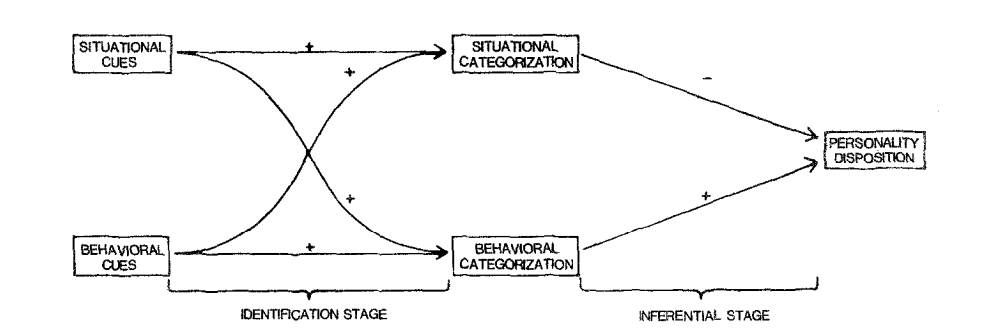
\includegraphics[width=\linewidth]{figures/TwoStageModel.png}
  \caption{Two-stage model according to Trope \cite{Trope1986}}
  \label{fig:twoStageModel}
\end{figure}

Another stream of research is concerned with why we form attributions.  In 1965, social psychologists Edward E. Jones and Keith Davis proposed an explanation for patterns of attribution termed correspondent inference theory. The basis for the inference is a correspondence between behaviour and disposition, according to the perceiver. They explained that certain conditions make us more likely to make a correspondent inference about someone's behaviour:

\begin{itemize}
\item Choice: If a behaviour is freely chosen it is believed to be due to internal (dispositional) factors.
\item Accidental vs. Intentional Behavior: Behavior that is intentional is likely to be attributed to the person’s personality, and behavior which is accidental is likely to be attributed to situation / external causes.
\item Social Desirability: Behaviors low in sociable desirability (non conforming) lead us to make (internal) dispositional inferences more than socially undesirable behaviors.  For example, if you observe a person getting on a bus and sitting on the floor instead of one of the seats. This behavior has low social desirability (non conforming) and is likely to correspond with the personality of the individual.
\item Hedonistic Relevance: If the other person’s behavior appears to be directly intended to benefit or harm us. 
\item Personalism: If the other person’s behavior appears to be intended to have an impact on us, we assume that it is “personal”, and not just a by-product of the situation we are both in.
\end{itemize}

% https://en.wikipedia.org/wiki/Correspondent_inference_theory
% https://www.simplypsychology.org/attribution-theory.html

% Other important work on attribution include covariance theory, https://en.wikipedia.org/wiki/Attribution_bias

Whereas people can make relatively logical assessments of cause and responsibility, as Heider predicted, researchers have found there are often systematic biases in how we make attributions \cite{Ross1977}. Perhaps the most well known bias is the fundamental attribution error, which is our tendency to make more internal attributions than external attributions for others’ behaviors. 

Considering the objectives of this thesis, our main goal lies not in measuring the fundamental attribution error directly, but rather in investigating the context of dispositional attribution. A focus on the fundamental attribution error, would require the employment of techniques of experimental social psychology. More realistically, we want to investigate whether a tendency to attribute dispositions exists. Nonetheless, studies around the fundamental attribution error are taken in consideration, as they contain relevant approaches and knowledge that could be of use when conducting the research for this thesis.  In a world in which the external environment rapidly changed, dispositional attributions might or might not look differently. 


